\begin{frame}
  \frametitle{Moment of Inertia (w.r.t. an axis)}

\begin{columns}[t]
  \column{7cm}
  $$I_L = \text{mass} \cdot \text{distance}^2 = M d^2$$

  For a lamina (thin )
  \begin{itemize}
    \item occupying a region $\mathcal{R}$,
    \item variable density $\rho \colon \mathcal{R} \to (0,\infty)$,
    \item distance to axis $h \colon \mathcal{R} \to [0,\infty)$, $h(P) = \text{distance}(P,L)$
  \end{itemize}
%
$$dI_L = h^2 \, dm = h^2\, \rho \, dA$$
%
$$I_L = \int\!\!\!\int_{\mathcal{R}} dI_L = \int\!\!\!\int_{\mathcal{R}} h^2 \; dm =\int\!\!\!\int_{\mathcal{R}} h^2 \, \rho \, dA$$
  \column{5.5cm}
     \begin{figure}
        \psfrag{L}{$L$}
        \psfrag{R}{$\mathcal{R}$}
        \psfrag{P}{$P$}
        \psfrag{hP}{$h(P)$}
        \psfrag{dA}{$\Delta A$}
        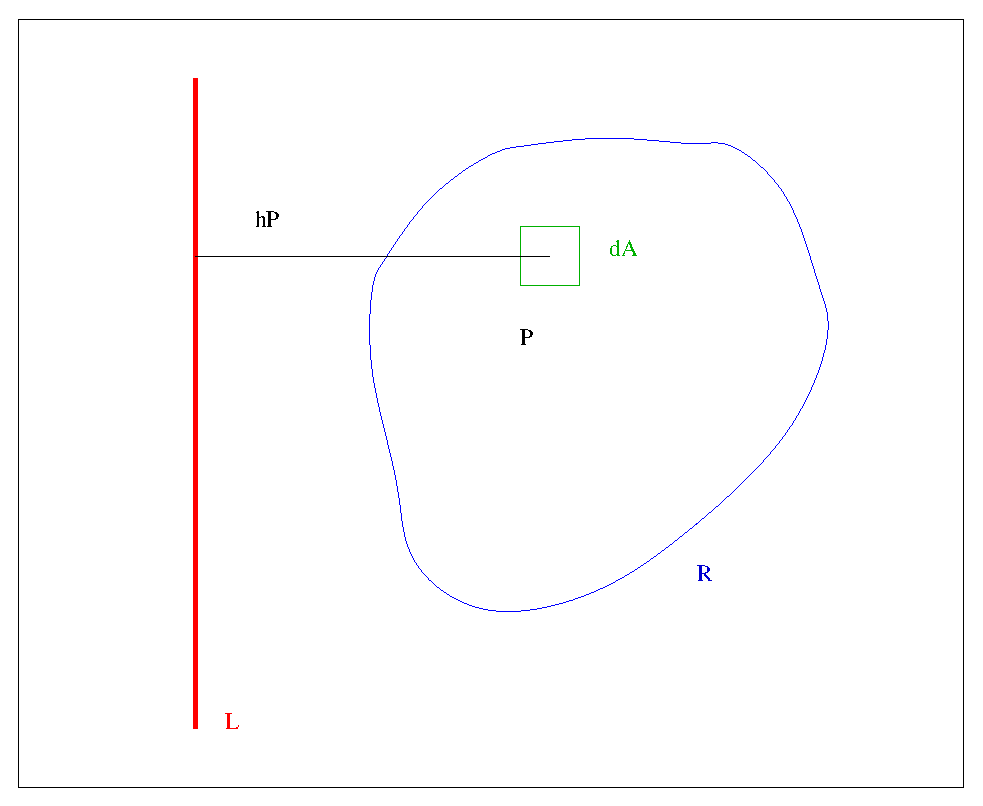
\includegraphics[width=2in]{../images/moment_inertia_lamina.eps}
    \end{figure}
\end{columns}
\end{frame}

\begin{frame}
\frametitle{Example}
\begin{columns}
  \column{7cm}
\only<1->{
Moment of inertia of a ring-like lamina with
\begin{itemize}
  \item inner radius $R_1$
  \item outer radius $R_2$
  \item and constant density $\rho$
\end{itemize}
about an axis that passes through its center:
%
$$I_L = \int\!\!\!\int_{\mathcal{R}} \rho\, h^2(P) dA \; .$$}

\only<2>{
In rectangular coordinates:
%
$$I_L = \int\!\!\!\int_{\mathcal{R}} \rho x^2 \; dx\,dy$$}

  \column{5.5cm}
  \only<1>{   \begin{figure}
        \psfrag{L}{$L$}
        \psfrag{R}{$\mathcal{R}$}
        \psfrag{P}{$P$}
        \psfrag{R1}{$R_1$}
        \psfrag{R2}{$R_2$}
        \includegraphics[width=2in]{../images/moment_inertia_ring.eps}
    \end{figure}}

   \only<2>{  \begin{figure}
        \psfrag{L}{$L$}
        \psfrag{R}{$\mathcal{R}$}
        \psfrag{P}{$P(x,y)$}
        \psfrag{R1}{$R_1$}
        \psfrag{R2}{$R_2$}
        \psfrag{O}{$O$}
        \psfrag{x}{$x$}
        \psfrag{y}{$y$}
        \psfrag{ax}{$|x|$}
        \includegraphics[width=2in]{../images/moment_inertia_ring_rectangular.eps}
    \end{figure}  }
\end{columns}

\end{frame}

\begin{frame}
  \frametitle{Computation in polar coordinates}

\begin{columns}
\column{6cm}
\only<1-3>{
\begin{figure}
        \psfrag{L}{$L$}
        \psfrag{R}{$\mathcal{R}$}
        \psfrag{P}{$P(x,y)$}
        \psfrag{R1}{$R_1$}
        \psfrag{R2}{$R_2$}
        \psfrag{O}{$O$}
        \psfrag{x}{$x$}
        \psfrag{y}{$y$}
        \psfrag{ax}{$|x|$}
        \includegraphics[width=2in]{../images/ring_region.eps}
    \end{figure}
    }

\only<4-6>{
\begin{figure}
        \psfrag{L}{$L$}
        \psfrag{R}{$\mathcal{R}$}
        \psfrag{P}{$P(x,y)$}
        \psfrag{R1}{$R_1$}
        \psfrag{R2}{$R_2$}
        \psfrag{O}{$O$}
        \psfrag{x}{$x$}
        \psfrag{y}{$y$}
        \psfrag{ax}{$|x|$}
        \includegraphics[width=2in]{../images/ring_region_divided.eps}
    \end{figure}
    }

\column{6cm}
\only<2>{
\begin{figure}
        \psfrag{R1}{$R_1$}
        \psfrag{R2}{$R_2$}
        \psfrag{0}{$0$}
        \psfrag{2p}{$2\pi$}
        \psfrag{r}{$r$}
        \psfrag{th}{$\theta$}
        \includegraphics[width=2in]{../images/ring_region_polar.eps}
    \end{figure}
}

\only<3-6>{
\begin{figure}
        \psfrag{R1}{$R_1$}
        \psfrag{R2}{$R_2$}
        \psfrag{0}{$0$}
        \psfrag{2p}{$2\pi$}
        \psfrag{r}{$r$}
        \psfrag{th}{$\theta$}
        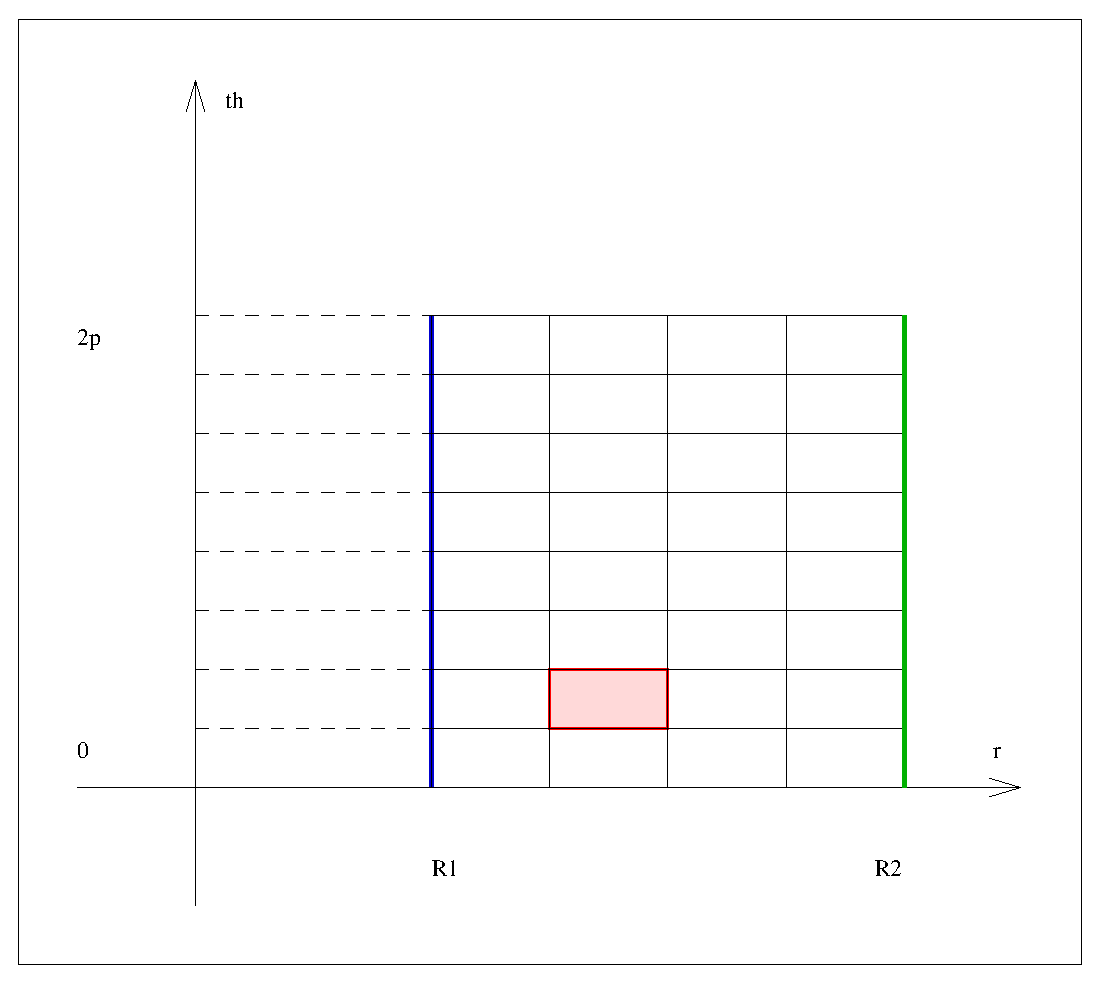
\includegraphics[width=2in]{../images/ring_region_polar_divided.eps}
    \end{figure}
}
\end{columns}
%
\begin{overlayarea}{\textheight}{5cm}
  \only<2>
  {
  $$\mathcal{R}_{polar} = [R_1,R_2] \times [0,\theta] = \{ (r,\theta) \, | \, R_1 \leqslant r \leqslant R_2, 0 \leqslant \theta \leqslant 2\pi\}$$
  }
  \only<3>
  {
  $$T \colon \mathcal{R}_{polar} \to \mathcal{R}_{rectangular}$$
  We divide the rectangular polar region into smaller rectangular polar regions, $D_1^p, \ldots, D_N^p$.
  }
  \only<4>
  {
  $$D_k = T(D_k^p)$$
  %
  The corresponding subregions of $\mathcal{R}$, for $k = 1,\ldots, N$ are regions that look like sectors of rings.
  }
  \only<5>
  {
  $$P_k = T(r_k,\theta_k)$$
  %
   For each subregion $D_k$ of $\mathcal{R}$, pick a sample point $P_k$ in $D_k$, and let $(r_k,\theta_k)$ be the corresponding point in the polar subregion $D_k^p$.
  }
  \only<6>{
  $$\int\!\!\!\int_{\mathcal{R}} f(P) dA \simeq \sum_{k=1}^N f(P_k)\cdot \text{area}(D_k) = \sum_{k=1}^N f(T(r_k,\theta_k))\cdot \text{area}(T(D_k^p)) \; .$$
  }
\end{overlayarea}
\end{frame}

\begin{frame}
\frametitle{Area Scaling}
\begin{figure}
        \psfrag{Tr1th}{$\textbf{T}(r,\theta)$}
        \psfrag{Tr2th}{$\textbf{T}(r+\Delta r,\theta)$}
        \psfrag{dthTth}{$(\Delta \theta)\textbf{T}_\theta(r,\theta)$}
        \psfrag{drTr}{$(\Delta r)\textbf{T}_r(r,\theta)$}
        \psfrag{x}{$x$}
        \psfrag{y}{$y$}
        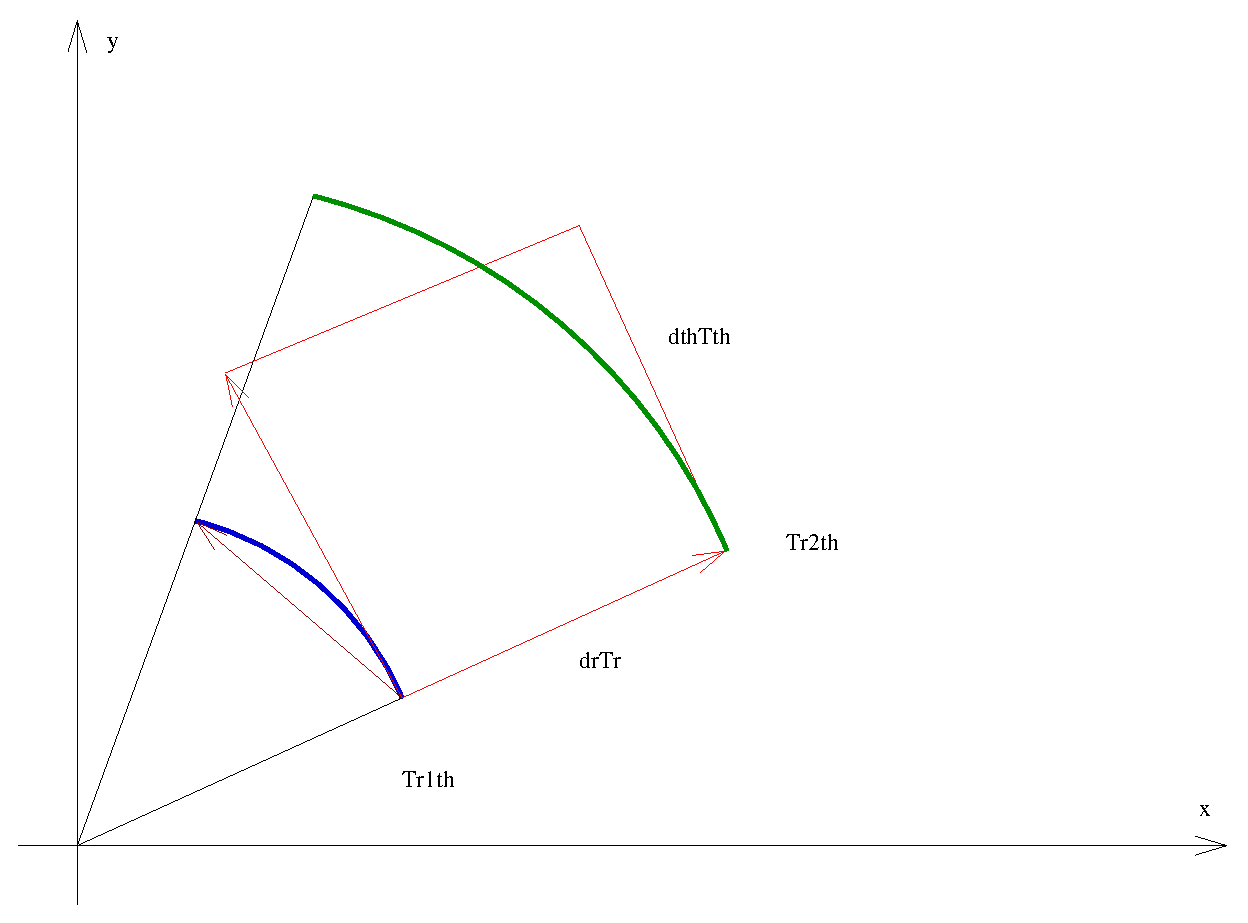
\includegraphics[width=2in]{../images/polar_element_area.eps}
    \end{figure}

$$\langle x, y \rangle = \textbf{T}(r,\theta) = \langle r\cos\theta, r\sin\theta\rangle$$
%
$$\textbf{T}(r+\Delta r,\theta)-\textbf{T}(r,\theta) \simeq (\Delta r) \textbf{T}_r(r,\theta)$$
%
$$\textbf{T}(r,\theta+\Delta \theta)-\textbf{T}(r,\theta) \simeq (\Delta \theta) \textbf{T}_\theta(r,\theta)$$
%
$$\text{Area}(D) \simeq |\textbf{T}_r \times \textbf{T}_\theta |\Delta r \Delta \theta =
\left|
\begin{array}{cc}
  \cos{\theta} & \sin{\theta} \\
  %
  -r\sin{\theta} & r\cos{\theta}
\end{array}
\right| \Delta r\, \Delta \theta = r\Delta r \Delta \theta \; .$$

\end{frame}

\begin{frame}
  \frametitle{Change of Variables}

  \begin{columns}
  \column{6cm}
  \begin{figure}
        \psfrag{L}{$L$}
        \psfrag{R}{$\mathcal{R}$}
        \psfrag{P}{$P(x,y)$}
        \psfrag{R1}{$R_1$}
        \psfrag{R2}{$R_2$}
        \psfrag{O}{$O$}
        \psfrag{x}{$x$}
        \psfrag{y}{$y$}
        \psfrag{ax}{$|x|$}
        \includegraphics[width=2in]{../images/ring_region_divided.eps}
    \end{figure}
  \column{6cm}
  \begin{figure}
        \psfrag{R1}{$R_1$}
        \psfrag{R2}{$R_2$}
        \psfrag{0}{$0$}
        \psfrag{2p}{$2\pi$}
        \psfrag{r}{$r$}
        \psfrag{th}{$\theta$}
        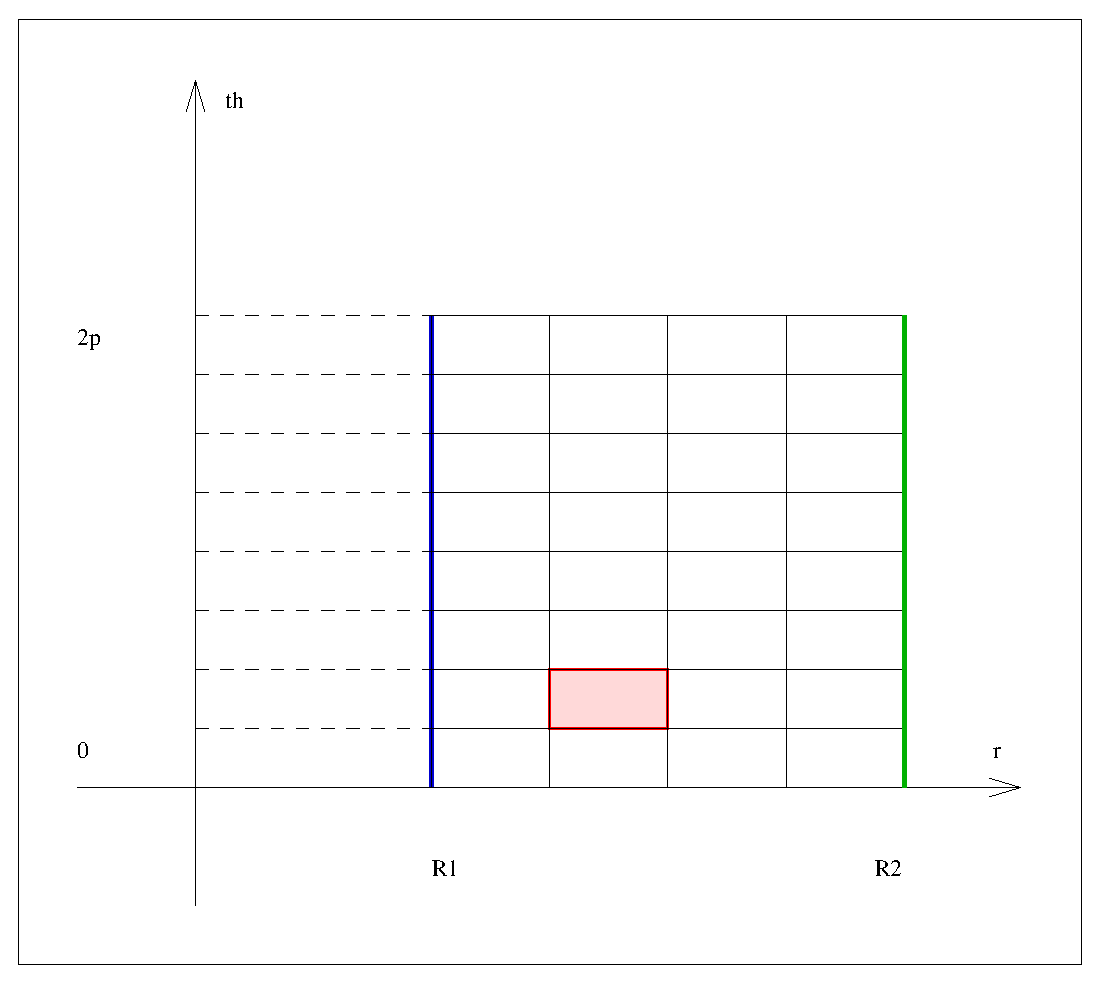
\includegraphics[width=2in]{../images/ring_region_polar_divided.eps}
    \end{figure}
  \end{columns}

  $$\int\!\!\!\int_{\mathcal{R}} f(P) dA \simeq \sum_{k=1}^N f(P_k)\cdot \text{area}(D_k) = \sum_{k=1}^N f(T(r_k,\theta_k))\cdot  r_k \Delta r \Delta \theta\; .$$
  %
$$\int\!\!\!\int_{\mathcal{R}} f(P) dA = \int\!\!\!\int_{\mathcal{R}_{polar}} f(r\cos{\theta},r\sin{\theta})\;\cdot \,r\, dr\, d\theta \; .$$
\end{frame}

\begin{frame}
  \frametitle{Example, continued}
$$\int\!\!\!\int_{\mathcal{R}} f(P) dA = \int\!\!\!\int_{\mathcal{R}_{polar}} f(r\cos{\theta},r\sin{\theta})\;\cdot \,r\, dr\, d\theta \; .$$
%
  Returning to the computation of the moment of inertia we get
%
\begin{align*}
  I_L & = \int\!\!\!\int_{\mathcal{R}} f(P) dA =
  \int\!\!\!\int_{\mathcal{R}} x^2\rho \, dxdy = \pause
  \int\!\!\!\int_{\mathcal{R}_{polar}}\!\!\!\! \rho (r\cos\theta)^2 \cdot r \, dr\, d\theta = \\ & =  \int\!\!\!\int_{[R_1,R_2] \times [0,2\pi]} \rho r^3\cos^2{\theta} \, dr\, d\theta =  \\ \pause & = \rho \left( \int_{r=R_1}^{r=R_2} r^3 \; dr \right) \left( \int_{\theta=0}^{\theta=2\pi} \frac{1+\cos{2\theta}}{2} \; d\theta \right)  = \\
  & = \frac{\pi \rho (R_2^4-R_1^4)}{4} = \rho \pi (R_2^2-R_1^2) \cdot \frac{R_1^2+R_2^2}{4} = \frac{m(R_1^2+R_2^2)}{4}\; .
\end{align*}
\end{frame}

\begin{frame}
  \frametitle{General Set-up}
 %
$$\int\!\!\!\int_{\mathcal{R}} f(P) \, dA\; .$$
%
The general method is the following:
%
\begin{itemize}
    \item \pause Choose a convenient polar coordinate system;
  \item \pause Change the \textcolor[rgb]{0.98,0.00,0.00}{region} $\mathcal{R}$ to
      %
      $$\mathcal{R}_{polar} = \{(r,\theta) \, | \, T(r,\theta) \in \mathcal{R} \}\, ,$$
      %
      the region of polar coordinates corresponding to points in $\mathcal{R}$.
      %
  \item \pause Change the \textcolor[rgb]{0.00,0.00,1.00}{function} $f\colon \mathcal{R} \to \mathbb{R}$ to $g \colon \mathcal{R}_{polar} \to \mathbb{R}$, $g(r,\theta) = f(T(r,\theta))$.
  \item \pause Change the \textcolor[rgb]{0.00,0.59,0.00}{element of area} $dA$ to $r dr d\theta$.
\end{itemize}
%
\pause Then
%
$$\int\!\!\!\int_{\textcolor[rgb]{0.98,0.00,0.00}{\mathcal{R}}} \textcolor[rgb]{0.00,0.00,1.00}{f(P)} \, \textcolor[rgb]{0.00,0.59,0.00}{dA}\; = \int\!\!\!\int_{\textcolor[rgb]{0.98,0.00,0.00}{\mathcal{R}_{polar}}} \textcolor[rgb]{0.00,0.00,1.00}{g(r,\theta)} \cdot \textcolor[rgb]{0.00,0.59,0.00}{r\,dr\,d\theta} \; .$$
\end{frame}

\begin{frame}
  \frametitle{Change of Coordinates}

  In many cases, the region $\mathcal{R}$ is given in rectangular coordinates, $\mathcal{R}_{rectangular}$ and the integral is
%
$$\int\!\!\!\int_{\mathcal{R}_{rectangular}} \!\!\!\!\! f(x,y) \, dxdy\; .$$
%
To change to polar coordinates:
%
$$\int\!\!\!\int_{\textcolor[rgb]{0.98,0.00,0.00}{\mathcal{R}_{rectangular}}} \!\!\!\!\! \textcolor[rgb]{0.00,0.00,1.00}{f(x,y)} \, \textcolor[rgb]{0.00,0.59,0.00}{dxdy} \rightsquigarrow
\int\!\!\!\int_{\textcolor[rgb]{0.98,0.00,0.00}{\mathcal{R}}}  \textcolor[rgb]{0.00,0.00,1.00}{f(P)} \, \textcolor[rgb]{0.00,0.59,0.00}{dA} \rightsquigarrow
\int\!\!\!\int_{\textcolor[rgb]{0.98,0.00,0.00}{\mathcal{R}_{polar}}} \!\!\!\!\! \textcolor[rgb]{0.00,0.00,1.00}{g(r,\theta)} \, \textcolor[rgb]{0.00,0.59,0.00}{r\,drd\theta} \; .$$

Strategy:
\begin{itemize}
  \item Change \textcolor[rgb]{0.98,0.00,0.00}{region} $\mathcal{R}_{rectangular} \to \mathcal{R} \to \mathcal{R}_{polar}$;
  %
  \item Change \textcolor[rgb]{0.00,0.00,1.00}{function} $f(x,y) \to f(r\cos\theta,r\sin\theta) = g(r,\theta)$;
  %
  \item Change \textcolor[rgb]{0.00,0.59,0.00}{element of area}: $dxdy \to r\,drd\theta$.
\end{itemize}
\end{frame}

\begin{frame}
  \frametitle{When Do We Use Polar Coordinates?}
  $$\int\!\!\!\int_{\mathcal{R}_{rectangular}} \!\!\!\!\! f(x,y) \, dxdy \rightsquigarrow
\int\!\!\!\int_{\mathcal{R}}  f(P) \, dA \rightsquigarrow
\int\!\!\!\int_{\mathcal{R}_{polar}} \!\!\!\!\! g(r,\theta) \, r\,drd\theta \; .$$
%
General Philosophy:
\begin{quote}
  The integral in polar coordinates should be easier
\end{quote}
%
\begin{itemize}
  \item \pause $\mathcal{R}_{polar}$ is a nice region. Examples:
  %
  \begin{itemize}
    \item \pause $\mathcal{R}_{polar} = [0,R] \times [0,2\pi]$ $\Longrightarrow$ $\mathcal{R}=$ \pause disk.
    %
    \item \pause $\mathcal{R}_{polar} = [R_1,R_2] \times [0,2\pi]$ $\Longrightarrow$ $\mathcal{R}=$ \pause ring;
    %
    \item \pause $\mathcal{R}_{polar} = [0,R] \times [\theta_1,\theta_2]$ $\Longrightarrow$ $\mathcal{R}=$ \pause sector of disk;
    %
    \item \pause $\mathcal{R}_{polar} = [R_1,R_2] \times [\theta_1,\theta_2]$ $\Longrightarrow$ $\mathcal{R}=$ \pause sector of ring;
        %
  \end{itemize}
  %
  \item \pause $r\, g(r,\theta) = r \,f(r\cos\theta, r\sin\theta)$ is not too complicated.
\end{itemize}
\end{frame}


\begin{frame}
  \frametitle{Example}

  Let $\mathcal{R}=\mathcal{R}_{rectangular}$ be the region left of $y-$axis and between the circles $x^2+y^2=1$ and $x^2+y^2=4$.  Compute
%
$$\int\!\!\!\int_{\mathcal{R}} (x+y)\, dxdy\; .$$

\begin{itemize}
  \item \pause The polar \textcolor[rgb]{0.98,0.00,0.00}{region} is
    %
    $$\mathcal{R}_{polar} = \{(r,\theta) \; | \; 1 \leqslant r \leqslant 2, \pi/2 \leqslant \theta \leqslant 3\pi/2 \} = [1,2]\times [\pi/2, 3\pi/2]\; .$$
    %
    \item \pause The \textcolor[rgb]{0.00,0.00,1.00}{function} is
    %
    $$g(r,\theta) = x+y = r\cos\theta+r\sin\theta = r(\cos\theta+\sin\theta)\; .$$
    %
    \item \pause The \textcolor[rgb]{0.00,0.59,0.00}{element of area} is $dxdy=r\, drd\theta$.
\end{itemize}

\pause Then the integral is
%
\begin{align*}
  \int&\!\!\!\int_{\textcolor[rgb]{0.98,0.00,0.00}{\mathcal{R}}} \textcolor[rgb]{0.00,0.00,1.00}{(x+y)}\, \textcolor[rgb]{0.00,0.59,0.00}{dxdy} = \int\!\!\!\int_{\textcolor[rgb]{0.98,0.00,0.00}{[1,2]\times [\pi/2, 3\pi/2]}} \!\!\!\!\! \textcolor[rgb]{0.00,0.00,1.00}{(r \cos\theta + r\sin\theta)} \cdot \textcolor[rgb]{0.00,0.59,0.00}{r dr\, d\theta} = \\
  %
  & = \left( \int_1^2 r^2\, dr \right)\left( \int_{\pi/2}^{3\pi/2} (\sin\theta+ \cos\theta) \, d\theta \right) = -\frac{14}{3}\; .
\end{align*}
\end{frame}

\begin{frame}
  \frametitle{Improper Integrals in Polar Coordinates}

  $\mathcal{Q}$: first quadrant, $[0,\infty) \times [0,\infty)$. Compute
%
$$\int\!\!\!\int_Q e^{-x^2-y^2} \, dxdy$$
%
\pause
%
\begin{align*}
  \int& \!\!\!\int_{\textcolor[rgb]{0.98,0.00,0.00}{\mathcal{Q}}} \textcolor[rgb]{0.00,0.00,1.00}{e^{-x^2-y^2}} \, \textcolor[rgb]{0.00,0.59,0.00}{dx \,dy}  = \pause \int\!\!\!\int_{\textcolor[rgb]{0.98,0.00,0.00}{[0,\infty) \times [0,\pi/2]}} \textcolor[rgb]{0.00,0.00,1.00}{e^{-r^2}} \, \textcolor[rgb]{0.00,0.59,0.00}{r\, dr \,d\theta} = \\
   %
    & = \left( \int_{\theta=0}^{\theta=\pi/2} d\theta \right) \left( \int_{r=0}^{r\to \infty} re^{-r^2} \, dr \right) = \frac{\pi}{2} \left. \frac{-e^{-r^2}}{2}\right|_{r=0}^{r\to \infty} = \frac{\pi}{4}\; .
\end{align*}
%
\pause \underline{Application}:
%
$$\frac{\pi}{4} = \int\!\!\!\int_{[0,\infty) \times [0,\infty)} e^{-x^2}\, e^{-y^2}\, dxdy = \left( \int_0^\infty e^{-x^2} dx \right) \left( \int_0^\infty e^{-y^2} dy \right)$$

$$\int_{-\infty}^{\infty} e^{-x^2} \, dx = \pause 2 \int_0^{\infty} e^{-x^2} \, dx = 2\left( \int \!\!\!\int_{\mathcal{Q}_1} e^{-x^2-y^2} \, dx \,dy \right)^{1/2} = \sqrt{\pi} \; .$$
\end{frame} 

\begin{frame}
  \frametitle{Moment of Inertia}

  Moment of inertia with respect to an axis $L$:
%
$$I_L = \text{mass} \cdot \text{distance}^2$$

\underline{Example}:  
\begin{itemize}
\item Homogeneous cylindrical shell $\mathcal{R}$;
\begin{itemize}
\item inner radius $R_1$, outer radius $R_2$ and height $H$
\end{itemize}
\item with respect to the axis $L$ of the cylinder.
\end{itemize}

If $h \colon \mathcal{R} \to [0,\infty)$ is the distance function, $h(P) = \text{distance}(P,L)$, then
%
$$dI_L = h^2 \, dm = h^2\, \rho \, dV$$
%
hence
%
$$I_L = \int\!\!\!\int\!\!\!\int_{\mathcal{R}} dI_L = \int\!\!\!\int\!\!\!\int_{\mathcal{R}} h^2 \; dm =\int\!\!\!\int\!\!\!\int_{\mathcal{R}} h^2 \, \rho \, dV = \int_{z=0}^{z=H} \left( \int\!\!\!\int_{D_z} \rho h^2 \, dA \right) \, dz \, $$
\end{frame}

\begin{frame}
  \frametitle{Cylindrical Coordinates}
  
%
\begin{itemize}
  \item Sections perpendicular to the axis $L$ are rings;
  \item Double integrals over such regions $\to$ use polar coordinates;
  \item Rectangular-polar coordinates $\to$ cylindrical coordinates $(r,\theta,z)$
\end{itemize}
%
Slice $D_z$: ring with inner radius $R_1$ and outer radius $R_2$. In polar coordinates:

\begin{itemize}
\item $D_z$ $\to$ $[R_1,R_2] \times [0,2\pi]$;
\item  $dA = r\, dr d\theta$;
\item $h(P) = r$
\end{itemize}

%
\begin{align*}
  I_L & = \int_{z=0}^{z=H} \left(
  \int\!\!\!\int_{[R_1,R_2] \times [0,2\pi]} \rho r^2 \, r\, dr\, d\theta \right) \, dz =\\
  %
  & = \int_{z=0}^{z=H} \left(
  \int_{r=R_1}^{r=R_2} \left(\int_{\theta=0}^{\theta=2\pi} \rho r^3 \, d\theta \right) \, dr\right) \, dz = 2\pi \rho H \frac{R_2^4-R_1^4}{4} = \\
  %
  &= \rho \pi (R_2^2-R_1^2)H \cdot \frac{R_1^2+R_2^2}{2} = \frac{m(R_1^2+R_2^2)}{2}\; .
\end{align*}
\end{frame}

\begin{frame}
    \frametitle{General Set-up}
%
$$\int\!\!\!\int\!\!\!\int_{\mathcal{R}} f(P) \, dV\; .$$
%
\underline{Step 1}: Choose a suitable cylindrical coordinate system: $(x,y,z) = T(r, \theta, z)$.

\underline{Step 2}: Change the region $\mathcal{R}$ to
      %
      $$\mathcal{R}_{cylindrical} = \{(r,\theta,z) \, | \, T(r,\theta,z) \in \mathcal{R} \}\, ,$$
      %

\underline{Step 3}: Change the function $f\colon \mathcal{R} \to \mathbb{R}$ to $g \colon \mathcal{R}_{cylindrical} \to \mathbb{R}$,
      %
      $$g(r,\theta,z) = f(T(r,\theta,z))\; .$$

\underline{Step 4}: Change the element of volume $dV$ to $ (dA)_{polar} \, dz = r \,dr\, d\theta \, dz$.
%
$$\int\!\!\!\int\!\!\!\int_{\mathcal{R}} f(P) \, dV\; = \int\!\!\!\int\!\!\!\int_{\mathcal{R}_{cylindrical}} g(r,\theta,z) \cdot r\,dr\,d\theta\, dz \; .$$

This method is efficient as long as the region $\cR_{cylindrical}$ is nice enough and the function $rg(r,\theta,z)$ is not too complicated.

\end{frame}

\begin{frame}
  \frametitle{Example: Center of Mass}

\begin{itemize}
\item solid conical body $\cR$ of radius $R$ and height $H$;
\item with density $\rho \colon \cR \to \RR$ proportional to the distance to the axis.
\end{itemize}
 
The position vector of the center of mass is
%
$$\textbf{r}_C = \frac{1}{M} \int\!\!\!\int\!\!\!\int_{\cR} \textbf{r} \; dm = \frac{1}{M} \int\!\!\!\int\!\!\!\int_{\cR} \textbf{r} \; \rho \; dV\; ,$$
%
where
%
$$M = \int\!\!\!\int\!\!\!\int_{\cR}  dm = \int\!\!\!\int\!\!\!\int_{\cR}  \rho(P) \, dV$$
%
is the mass of the body.

  Region best described in a coordinate system
  \begin{itemize}
    \item rectangular in one direction
    \item polar on the orthogonal complement
  \end{itemize}
  %
  Cylindrical coordinates!
\end{frame}

\begin{frame}
  \frametitle{Set-up in Cylindrical Coordinates}

\underline{Step 1}: Choose a suitable cylindrical coordinate system: $(x,y,z) = T(r, \theta, z)$.
%
\begin{itemize}
\item origin at the vertex of the cone;
\item positive $z-$axis along the axis of the cone.
\end{itemize}

\underline{Step 2}: Change the region $\mathcal{R}$ to
      %
      $$\mathcal{R}_{cylindrical} = \{(r,\theta,z) \, | \, T(r,\theta,z) \in \mathcal{R} \}\, ,$$
      %
      \begin{itemize}
      \item the base is the disk $D$ with center on the $z-$axis and radius $R$ in the plane $z=H$;
      \item the cone is given by $z= \frac{H}{R}\,r$.
      \end{itemize}
      %
$$\cR_{cylindrical} = \left\{ (r,\theta,z) \; | \; 0 \leqslant \theta \leqslant 2\pi, 0 \leqslant r \leqslant R, \frac{H}{R} \,r \leqslant z \leqslant H\right\} \, .$$
      
      \end{frame}
      
 \begin{frame}
\underline{Step 3}: Change the density $\rho(P)$ to $g \colon \mathcal{R}_{cylindrical} \to \mathbb{R}$,
      %
      $$g(r,\theta,z) = f(T(r,\theta,z)) =  cr\; .$$

\underline{Step 4}: Change the element of volume $dV$ to $ (dA)_{polar} \, dz = r \,dr\, d\theta \, dz$.
%
$$\int\!\!\!\int\!\!\!\int_{\mathcal{R}} f(P) \, dV\; = \int\!\!\!\int\!\!\!\int_{\mathcal{R}_{cylindrical}} g(r,\theta,z) \cdot r\,dr\,d\theta \, dz \; .$$

Then
%
\begin{align*}
  M & = \int\!\!\!\int\!\!\!\int_{\cR} \rho(P) \, dV = \int\!\!\!\int\!\!\!\int_{\cR_{cylindrical}} \!\!\!\!\! cr \cdot r\,dr\,d\theta\,dz = \\
%
  & = \int\!\!\!\int_{D} \left( \int_{z=Rr/R}^{z=H} \rho(r,\theta,z) \, dz \right) \, dA \\
  %
  & = \int\!\!\!\int_{[0,R]\times [0,2\pi]} \left( \int_{z=Hr/R}^{z=H} cr^2 dz \right) \, dr\, d\theta = \\
  %
  & = \int_{\theta =0}^{\theta=2\pi} \left( \int_{r=0}^{r=R} \left( \int_{z=Hr/R}^{z=H} cr^2 \, dz \right) \, dr \right) \, d\theta  = \frac{\pi c H R^3}{6}\; .
\end{align*}
%
\end{frame}

\begin{frame}
  \frametitle{Center of Mass}

$$M = \frac{\pi c H R^3}{6}\; .$$

Dimensional analysis:
%
$$\rho = c r \Longrightarrow [m/d^3] = [c][d] \Longrightarrow [c] = [m/d^4] \Longrightarrow [M] = [m/d^4][d^4] = [m] \;  $$
%

\begin{itemize}
\item region is symmetrical with respect to the axis of the cone;
\item distribution of mass is symmetrical with respect to the axis of the cone
\end{itemize}

Therefore the center of mass is also on this axis!

%
\begin{align*}
  z_C & = \frac{1}{M}  \int\!\!\!\int\!\!\!\int_{\cR} z \rho(P) \, dV = \frac{1}{M} \int_{\theta =0}^{\theta=2\pi} \left( \int_{r=0}^{r=R} \left( \int_{z=Hr/R}^{z=H} cr^2z \, dz \right) \, dr \right) \, d\theta = \\
  %
  & = \frac{6}{\pi c H R^3}\cdot \frac{2\pi c H^2 R^3}{15} = \frac{4}{5}\, H\; .
\end{align*}
\end{frame}

\begin{frame}
\frametitle{Area Scaling}
\begin{figure}
        \psfrag{Tr1th}{$\textbf{T}(r,\theta)$}
        \psfrag{Tr2th}{$\textbf{T}(r+\Delta r,\theta)$}
        \psfrag{dthTth}{$(\Delta \theta)\textbf{T}_\theta(r,\theta)$}
        \psfrag{drTr}{$(\Delta r)\textbf{T}_r(r,\theta)$}
        \psfrag{x}{$x$}
        \psfrag{y}{$y$}
        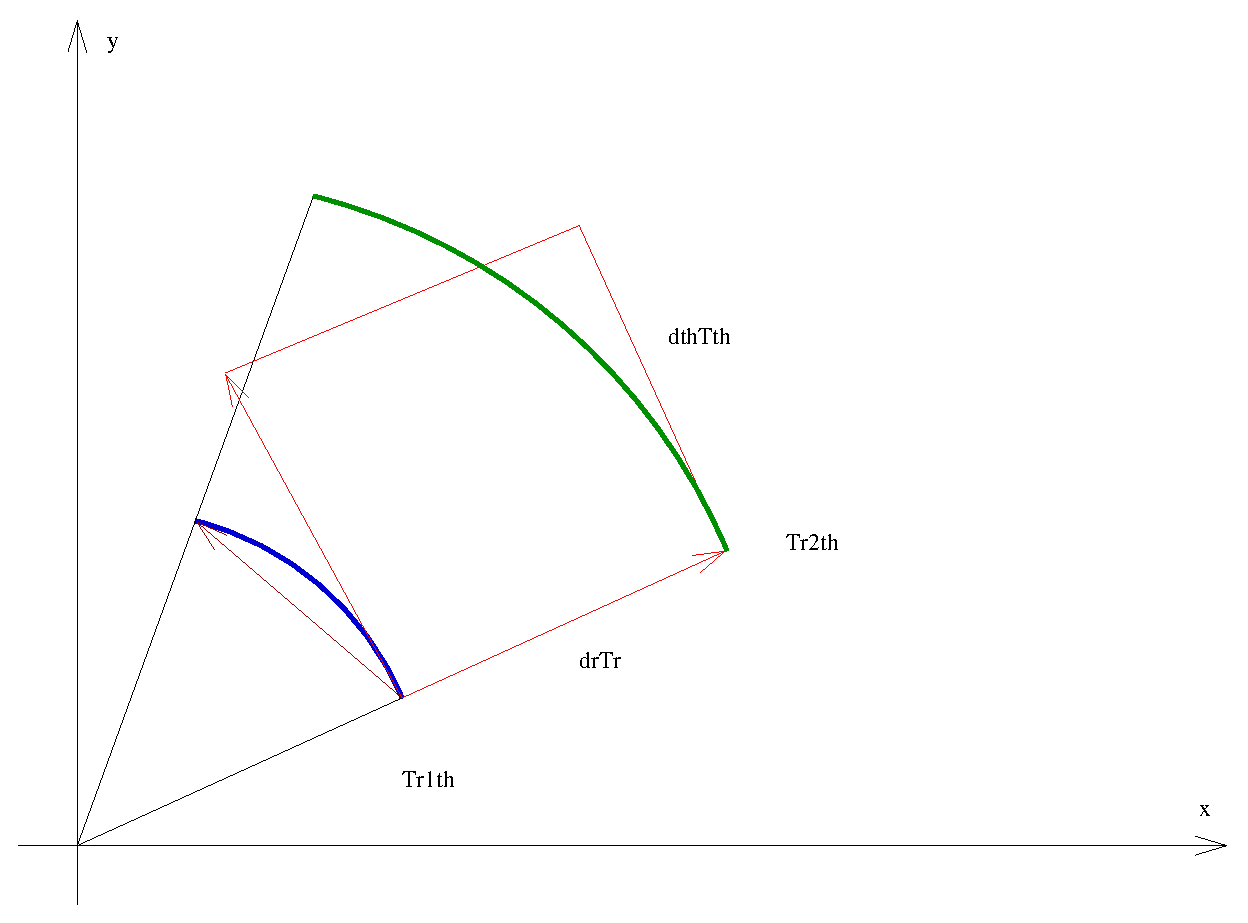
\includegraphics[width=2in]{../images/polar_element_area.eps}
    \end{figure}
%
$$\langle x, y \rangle = \textbf{T}(r,\theta) = \langle r\cos\theta, r\sin\theta\rangle$$
%
$$\textbf{T}(r+\Delta r,\theta)-\textbf{T}(r,\theta) \simeq (\Delta r) \textbf{T}_r(r,\theta)$$
%
$$\textbf{T}(r,\theta+\Delta \theta)-\textbf{T}(r,\theta) \simeq (\Delta \theta) \textbf{T}_\theta(r,\theta)$$
%
$$\text{Area}(D) \simeq |\textbf{T}_r \times \textbf{T}_\theta |\Delta r \Delta \theta =
\left|
\begin{array}{cc}
  \cos{\theta} & \sin{\theta} \\
  %
  -r\sin{\theta} & r\cos{\theta}
\end{array}
\right| \Delta r\, \Delta \theta = r\Delta r \Delta \theta \; .$$
%
$$dx\,dy = r dr\, d\theta\; .$$
%
\end{frame}


\begin{frame}
    \frametitle{Element of volume in spherical coordinates}

$T$:  transformation from spherical to rectangular coordinates:
%
$$(x,y,z) = T(\rho, \phi, \theta) = (\rho \sin\phi \cos\theta, \rho \sin\phi\sin\theta, \rho \cos\phi)\; .$$
%
Then
%
\begin{align*}
  \textbf{T}_{\rho} = & \langle \sin\phi \cos\theta, \sin\phi\sin\theta, \cos\phi\rangle \\
  \textbf{T}_{\phi} = & \langle \rho\cos\phi \cos\theta, \rho\cos\phi\sin\theta, - \rho\sin\phi\rangle \\
  \textbf{T}_{\theta} = & \langle -\rho \sin\phi \sin\theta, \rho \sin\phi\cos\theta, 0\rangle
\end{align*}
%
hence
%
$$J(T) = \textbf{T}_{\rho} \cdot (\textbf{T}_{\phi} \times \textbf{T}_{\theta}) = \left|
\begin{array}{ccc}
  \sin\phi \cos\theta &  \sin\phi\sin\theta & \cos\phi \\
  %
  \rho\cos\phi \cos\theta & \rho\cos\phi\sin\theta & - \rho\sin\phi \\
  %
  -\rho \sin\phi \sin\theta &  \rho \sin\phi\cos\theta & 0
\end{array}\right| = \rho^2\sin\phi\; .$$
%
$$dx\, dy\, dz = dV = \rho^2\sin\phi\,  d\rho\, d\phi\, d\theta\; .$$
\end{frame}

\begin{frame}
    \frametitle{Example: Centroid of a hemispherical region}

Coordinate system: 
%
\begin{itemize}
\item Origin: center of the sphere;
\item $Oxy$ plane: base of the hemisphere.
\item $Oz$ axis: towards the hemisphere
\item Spherical coordinates: $(\rho, \phi, \theta)$.
\end{itemize}

Region symmetric with respect to the $z-$axis: the centroid is on that axis $\to$ $x_C=y_C=0$. 

The $z-$coordinate is
%
$$z_C = \frac{1}{\text{Vol}(\cR)} \int\!\!\!\int\!\!\!\int_{\cR} z\, dV\; .$$
%
Spherical coordinate \textcolor[rgb]{0.98,0.00,0.00}{region}:
%
$$\textcolor[rgb]{0.98,0.00,0.00}{\cR_{spherical}} = \{ (\rho, \phi, \theta) \; | \; 0 \leqslant \rho \leqslant R,\; 0 \leqslant \phi \leqslant \frac{\pi}{2}, \; 0 \leqslant \theta \leqslant 2\pi \}\; ;$$
%
\textcolor[rgb]{0.00,0.00,0.98}{Function}:
%
$$z= \textcolor[rgb]{0.00,0.00,0.98}{\rho \cos\phi} \; ;$$
%
\textcolor[rgb]{0.00,0.98,0.00}{Element of volume}:
%
$$dV = \textcolor[rgb]{0.00,0.98,0.00}{\rho^2 \sin\phi \, d\rho\, d\phi\, d\theta}\; ;$$
\end{frame}

\begin{frame}
\frametitle{Set-up}

Therefore
%
\begin{align*}
  z_C & = \frac{1}{\text{Vol}(\cR)} \int\!\!\!\int\!\!\!\int_{\textcolor[rgb]{0.98,0.00,0.00}{\cR}} \textcolor[rgb]{0.00,0.00,0.98}{z}\, \textcolor[rgb]{0.00,0.98,0.00}{dV}\;  \\
  & = \frac{3}{2\pi R^3} \int\!\!\!\int\!\!\!\int_{\textcolor[rgb]{0.98,0.00,0.00}{\cR_{spherical}}} \textcolor[rgb]{0.00,0.00,0.98}{\rho \cos\phi} \cdot 
  \textcolor[rgb]{0.00,0.98,0.00}{\rho^2\sin\phi \, d\rho\, d\phi\,d\theta} \\
  %
  & = \frac{3}{2\pi R^3} \int_{\theta =0}^{\theta=2\pi} \left(
  \int_{\phi = 0}^{\phi=\pi/2} \left(
  \int_{\rho = 0}^{\rho = R} \rho^3 \sin\phi\cos\phi \, d\rho
  \right) \, d\phi
  \right) \, d\theta  \\
  & = \frac{3}{2\pi R^3} \left(\int_{\theta =0}^{\theta=2\pi} d\theta \right) \left( \int_{\phi = 0}^{\phi=\pi/2} \sin\phi\cos\phi\, d\phi \right) \left( \int_{\rho = 0}^{\rho = R} \rho^3 \, d\rho \right)  \\
  %
  & = \frac{3}{2\pi R^3} \cdot 2\pi \cdot \left( \left. \frac{1}{2}\sin^2\phi \right|_{\phi=0}^{\phi=\pi/2}\right) \cdot \left( \left. \frac{\rho^4}{4} \right|_{\rho=0}^{\rho=R} \right) = \frac{3}{8} \, R\; .
\end{align*}
\end{frame}







